\documentclass[11pt,a4paper]{article}

% Pacotes essenciais
\usepackage[utf8]{inputenc}
\usepackage[T1]{fontenc}
\usepackage{lmodern}
\usepackage[portuguese]{babel}
\usepackage{graphicx}
\usepackage{amsmath}
\usepackage{amsfonts}
\usepackage{amssymb}
\usepackage{float}
\usepackage{caption}
\usepackage{subcaption}
\usepackage{xcolor}
\usepackage{fancyhdr}
\usepackage{geometry}
\usepackage{titlesec}
\usepackage{cite}
\usepackage{booktabs}
\usepackage{array}
\usepackage{tikz}
\usepackage[hidelinks]{hyperref}
\usepackage{lastpage}

% Definição das cores
\definecolor{headercolor}{HTML}{b11116}
\definecolor{secondarycolor}{HTML}{3a5461}

% Configuração da página
\geometry{
    a4paper,
    top=2.8cm,
    bottom=2.5cm,
    left=2.5cm,
    right=2.5cm,
    headheight=1.2cm,
    headsep=0.5cm
}

% Configuração do cabeçalho
\pagestyle{fancy}
\fancyhf{}
\renewcommand{\headrulewidth}{0pt}
\renewcommand{\footrulewidth}{0.5pt}

\fancyhead[L]{%
    \begin{tikzpicture}[remember picture, overlay]
        \fill[headercolor] (current page.north west) rectangle ([yshift=-1.2cm]current page.north east);
        \node[anchor=west, inner sep=0pt] at ([xshift=1cm, yshift=-0.6cm]current page.north west) 
            {\includegraphics[height=0.8cm]{imgs/base/fatec-rgt.png}};
        \node[anchor=east, inner sep=0pt] at ([xshift=-1cm, yshift=-0.6cm]current page.north east) 
            {\includegraphics[height=0.9cm]{imgs/base/cps-logo.png}};
        \node[anchor=east, inner sep=0pt] at ([xshift=-2.8cm, yshift=-0.6cm]current page.north east) 
            {\includegraphics[height=1.05cm]{imgs/base/governo-sp-secretaria-logo.png}};
    \end{tikzpicture}
}

\fancyfoot[L]{\footnotesize\textcolor{secondarycolor}{Faculdade de Tecnologia do Estado de São Paulo\\ fatecregistro.cps.sp.gov.br}}
\fancyfoot[R]{\thepage\ de \pageref{LastPage}}

% Configuração dos títulos das seções
\titleformat{\section}  
    {\normalfont\large\bfseries\color{secondarycolor}}
    {\thesection}{1em}{}

\titleformat{\subsection}
    {\normalfont\normalsize\bfseries\color{secondarycolor}}
    {\thesubsection}{1em}{}

% Informações do artigo
\title{\vspace{0.6cm}\textbf{\large Criação de Camarão em Cativeiro com Monitoramento IoT para Gastronomia} \\[0.2cm]
\large \textit{Shrimp Farming in Captivity with IoT Monitoring for Gastronomy}}

\author{
    Davi Mathais de Almeida$^{1}$, Leandro Augusto de Souza Muniz$^{1}$, Tiago de Lara Rodrigues$^{1}$ \\[0.3cm]
    \small
    $^{1}$Faculdade de Tecnologia do Estado de São Paulo \\
    \textit{davi.almeida@aluno.cps.sp.gov.br, leandro.muniz@aluno.cps.sp.gov.br,} \\
    \textit{tiago.rodrigues01@aluno.cps.sp.gov.br}
}
\date{}

\begin{document}

% Força o cabeçalho em todas as páginas
\pagestyle{fancy}

\maketitle
\thispagestyle{fancy}

% Resumo
\section*{Resumo}

A carcinicultura no Vale do Ribeira, em São Paulo, enfrenta desafios relacionados ao manejo predominantemente manual e à ausência de controle automatizado da alimentação e de registro histórico dos parâmetros da água, conforme relatado em pesquisa de campo exploratória. Para mitigar esses problemas, este trabalho desenvolveu um sistema de monitoramento e automação para cativeiros de camarão de água doce, integrando Internet das Coisas (IoT) a uma Aplicação Web Progressiva. O sistema utiliza um microcontrolador ESP32 com sensores de temperatura, pH e amônia, que enviam leituras a cada minuto, e um dispensador automatizado de ração. Os dados são armazenados em nuvem e disponibilizados em um painel interativo com histórico em gráficos, alertas por notificação \textit{push} e e-mail e configuração remota da alimentação. Testes de validação em escala de bancada, em um aquário com camarões \textit{Macrobrachium rosenbergii} e em amostras de sua água, indicaram erro absoluto médio de 0,37°C no sensor de temperatura e de 0,29 no de pH, com leituras sistematicamente abaixo da referência (precisão média de 98,27\% e 95,98\%, respectivamente). O monitoramento de amônia não foi validado e o alimentador funcionou como esperado. Conclui-se que a viabilidade técnica foi indicada, com o objetivo geral parcialmente alcançado e aprimoramentos necessários na validação da amônia e na resiliência a falhas de conectividade. A qualidade gastronômica do produto, que motiva o trabalho, não foi avaliada.

\vspace{0.3cm}
\noindent\textit{\textbf{Palavras-chave:}} Carcinicultura, Monitoramento, Internet das Coisas, Automação, Gastronomia, Vale do Ribeira.

\section*{Abstract}

Shrimp farming in the Vale do Ribeira, São Paulo, faces challenges related to predominantly manual management and the absence of automated feeding control and historical records of water parameters, as reported in an exploratory field survey. To mitigate these problems, this work developed a monitoring and automation system for captive freshwater shrimp farming, integrating the Internet of Things (IoT) with a Progressive Web Application. The system uses an ESP32 microcontroller with temperature, pH, and ammonia sensors that send readings every minute, and an automated feed dispenser. Data are stored in the cloud and made available on an interactive dashboard with historical graphs, push and e-mail alerts, and remote feeding configuration. Bench-scale validation tests, performed in an aquarium with \textit{Macrobrachium rosenbergii} shrimp and in samples of its water, indicated a mean absolute error of 0.37°C for the temperature sensor and 0.29 for the pH sensor, with readings systematically below the reference (mean precision of 98.27\% and 95.98\%, respectively). Ammonia monitoring was not validated, and the feeder worked as expected. It is concluded that technical feasibility was indicated, with the general objective partially achieved and improvements required in ammonia validation and resilience to connectivity failures. The gastronomic quality of the product, which motivates the work, was not evaluated.

\vspace{0.3cm}
\noindent\textit{\textbf{Keywords:}} Shrimp farming, Monitoring, Internet of Things, Automation, Gastronomy, Vale do Ribeira.

\vspace{0.5cm}
\noindent\rule{\textwidth}{0.5pt}
\vspace{0.5cm}

% Introdução
\section{Introdução}

Segundo \cite{bertini2021}, Caridea é um grupo de crustáceos amplamente conhecido como camarões, animais da ordem Decapoda, encontrados em ambientes de água doce ou salgada. Estima-se a existência de aproximadamente 3.500 espécies, distribuídas em 16 superfamílias e 36 famílias, sendo cerca de 800 de água doce e 2.700 de água salgada. A carcinicultura refere-se à criação de camarões em cativeiros, podendo ser aplicada a espécies marinhas ou de água doce.

A produção mundial de camarão tem crescido, em média, 4,97\% ao ano nos últimos sete anos, com o Equador como maior produtor e exportador, seguido por China, Índia, Vietnã, Indonésia, Tailândia e Brasil \cite{Rocha2023}. No Brasil, o camarão é a segunda maior fonte de valor na produção aquícola, concentrando-se principalmente na região Nordeste, com destaque para o Ceará, que registrou 43,7 mil toneladas em 2022. A região Nordeste responde por cerca de 99\% da produção brasileira, totalizando 92,4 mil toneladas no mesmo ano \cite{Ximenes2023}. No Brasil, a carcinicultura marinha predomina amplamente sobre a de água doce \cite{sebrae2018}, de modo que os números nacionais acima referem-se, em sua maior parte, ao camarão marinho. Para o cultivo de camarão de água doce, foco deste trabalho, não foram localizados dados específicos para o Vale do Ribeira.

O Vale do Ribeira, localizado no sul do estado de São Paulo, apresenta condições ambientais favoráveis à carcinicultura, como rios, estuários e manguezais, com produção concentrada nos municípios de Iguape, Cananeia e Sete Barras. Os camarões de água doce da região pertencem às famílias Palaemonidae e Atyidae, com destaque para os gêneros \textit{Palaemon}, \textit{Palaemonetes} e \textit{Macrobrachium} \cite{bertini2021}. A aquicultura de água doce, em especial a piscicultura, é uma atividade antiga na região \cite{castellani2005}, e, apesar do potencial produtivo, a atividade enfrenta desafios relacionados à má gestão dos cativeiros, infraestrutura limitada, poluição e proliferação de doenças, comprometendo a qualidade do produto e a rentabilidade.

A qualidade da água é um dos fatores determinantes para a produção de camarões com valor gastronômico. Variações inadequadas de temperatura podem causar estresse fisiológico nos camarões, afetando o metabolismo, o consumo de oxigênio e o desempenho produtivo \cite{praciano2018}. O pH inadequado prejudica a osmorregulação e degrada aminoácidos responsáveis pelo sabor do camarão \cite{Hsieh2021}, além de favorecer a proliferação de bactérias do gênero \textit{Vibrio}, que representam risco à saúde do consumidor \cite{han2025}. A amônia, produzida pelo metabolismo proteico e pela decomposição de matéria orgânica, provoca danos ao tecido muscular e ao hepatopâncreas em concentrações elevadas \cite{han2025}. Sistemas de rastreabilidade na aquicultura constituem um diferencial competitivo e um requisito crescente para acesso a mercados internacionais \cite{UniversoSaudeAnimal2025}. Nesse contexto, o monitoramento contínuo dos parâmetros do cativeiro é um requisito para manter a qualidade da água e, por consequência, o valor gastronômico do produto, motivação que orienta o desenvolvimento do sistema proposto neste trabalho.

Para entender as condições reais de manejo na região, foi conduzida uma pesquisa de campo com participantes vinculados à carcinicultura no Vale do Ribeira, por meio de entrevistas estruturadas com roteiro de dez questões voltadas às rotinas de manejo e aos cuidados com os cativeiros. Os resultados indicaram que o manejo é realizado de forma predominantemente manual, com os responsáveis dedicando em média cinco horas diárias ao cuidado dos cativeiros e realizando a verificação dos parâmetros da água de três a quatro vezes por dia, nos períodos da manhã, tarde e noite. Os participantes relataram que já ocorreram perdas de camarões tanto por falhas na alimentação, situações em que os animais deixaram de ser alimentados, quanto por alterações nos parâmetros da água, especialmente elevação da amônia, que se converte em nitrito e compromete a qualidade do ambiente aquático. A ausência de controle automatizado da alimentação e de registro histórico dos parâmetros da água foi apontada como principal fator que dificulta a identificação precoce de alterações críticas e aumenta o risco de perdas.

Nesse contexto, a Internet das Coisas (do inglês, \textit{Internet of Things}, ou IoT) tem se consolidado como uma abordagem promissora para o monitoramento e automação de sistemas aquícolas. A capacidade de coletar dados ambientais de forma contínua por meio de sensores conectados, transmiti-los para a nuvem e disponibilizá-los ao produtor de forma remota representa um avanço significativo em relação ao manejo manual tradicional. Estudos recentes demonstram que a adoção de sistemas baseados em IoT na carcinicultura contribui para o aumento da precisão no monitoramento da qualidade da água, a redução do tempo de resposta a alterações críticas e a melhoria dos indicadores produtivos, como taxa de sobrevivência e crescimento dos animais \cite{Uddin2020}. A integração dessas tecnologias à realidade dos produtores do Vale do Ribeira representa, portanto, uma oportunidade concreta de modernização da atividade com impacto direto na qualidade e na rentabilidade da produção.

Para superar esses desafios, é proposta a implementação de um sistema de monitoramento inteligente baseado em IoT. O sistema monitora parâmetros críticos, como temperatura, potencial hidrogeniônico (pH) e amônia, utilizando sensores conectados ao microcontrolador ESP32 com rede sem fio (\textit{Wi-Fi}) para coleta e transmissão contínua de dados. A aplicação web permite ao usuário visualizar informações, controlar remotamente as operações e acionar um alimentador automático programável, que distribui ração conforme horários e quantidades definidas. Além disso, o sistema gera relatórios históricos, gráficos e envia notificações preventivas em caso de alterações críticas, garantindo maior eficiência e segurança na criação de camarões.

% Objetivo
\section{Objetivos}

Este trabalho tem como objetivo desenvolver um sistema de monitoramento automatizado para cativeiros de camarão, integrando sensores IoT a uma aplicação web progressiva, a fim de auxiliar produtores no acompanhamento contínuo dos parâmetros da água e no controle da alimentação dos cativeiros.

\subsection{Objetivos específicos}
 
\begin{enumerate}
    \item Monitorar remotamente os parâmetros de temperatura, pH e amônia da água dos cativeiros, emitindo alertas automáticos ao usuário em caso de desvios nos valores esperados.
 
    \item Registrar e armazenar dados históricos dos cativeiros e das alimentações, disponibilizando relatórios e gráficos para análise das condições da água ao longo do tempo.
 
    \item Automatizar o fornecimento de ração por meio de um dispensador controlado pelo sistema, com horários e quantidades definidos pelo usuário.
    
    \item Desenvolver uma aplicação web progressiva e responsiva, adaptável a dispositivos móveis e \textit{desktop}, que disponibilize ao produtor acesso remoto aos parâmetros monitorados e à configuração da alimentação.
 
\end{enumerate}

% Estado da Arte
\section{Estado da Arte}
 
A utilização de sistemas de monitoramento baseados em IoT na carcinicultura tem sido explorada em diferentes contextos, com abordagens variadas quanto à tecnologia de comunicação, aos parâmetros monitorados e à forma de suporte à decisão.
 
O trabalho de \cite{dantas2020} propõe um sistema de telemonitoramento para a criação de camarões utilizando microcontroladores ESP32 integrados a módulos de Longo Alcance (do inglês, \textit{Long Range}, ou LoRa) e sensores de pH, oxigênio dissolvido e temperatura. A transmissão dos dados ocorre via Rede de Longo Alcance e Ampla Cobertura (do inglês, \textit{Long Range Wide Area Network}, ou LoRaWAN), com integração aos Serviços de Nuvem da Amazon (do inglês, \textit{Amazon Web Services}, ou AWS) por meio do Protocolo de Telemetria por Enfileiramento de Mensagens (do inglês, \textit{Message Queuing Telemetry Transport}, ou MQTT). A escolha do LoRaWAN foi motivada pela necessidade de cobrir grandes áreas rurais sem dependência de infraestrutura de rede local. Os resultados apresentaram medições precisas de temperatura e pH, com variações mínimas de 0,5°C, e alcance de comunicação de aproximadamente 138 metros, suficiente para fazendas de pequeno e médio porte. No entanto, o estudo apresenta limitações metodológicas significativas: a ausência de monitoramento de amônia ignora um dos principais fatores de mortalidade em cativeiros, enquanto a baixa autonomia energética do protótipo restringe sua viabilidade para implantações de longo prazo em cativeiros isolados, exigindo infraestrutura elétrica local contínua.
 
\cite{Uddin2020} apresenta um sistema de monitoramento em tempo real para fazendas de camarão de água doce (\textit{Macrobrachium rosenbergii}) em Bangladesh, integrando sensores de temperatura, pH, salinidade, oxigênio dissolvido e turbidez a um microcontrolador Arduino Yun. Os dados são transmitidos para uma camada de nuvem que aplica o método de Análise Hierárquica (do inglês, \textit{Analytic Hierarchy Process}, ou AHP), calculando um índice composto de qualidade da água que orienta o produtor sobre a necessidade de intervenção, com notificações automáticas via portal web. O sistema operou por 120 dias em ambiente real de cultivo, coletando mais de 4.600 registros com erro médio inferior a 7\% em relação a medições manuais de referência. A comparação entre um cativeiro monitorado pelo sistema IoT e outro gerenciado manualmente evidenciou ganhos expressivos na biometria e na taxa de sobrevivência (90\% contra 80--90\%). Como limitações críticas, a arquitetura depende exclusivamente de conectividade \textit{Wi-Fi}, o que representa um ``gargalo'' severo em zonas rurais, e a necessidade de calibração manual frequente dos sensores acaba por mitigar os ganhos de tempo proporcionados pela automação, exigindo intervenção humana constante.
 
O trabalho de \cite{Arifani2024} propõe um protótipo de monitoramento da qualidade da água para a criação de camarões Vannamei utilizando um microcontrolador Arduino Uno acoplado a um NodeMCU ESP8266, integrados aos sensores DS18B20 (temperatura), PH SEN0161 (pH) e um sensor de Sólidos Totais Dissolvidos (do inglês, \textit{Total Dissolved Solids}, ou TDS) para condutividade. A comunicação entre os dois microcontroladores ocorre via porta serial, com o ESP8266 responsável por transmitir os dados via Wi-Fi diretamente para o Google Planilhas (\textit{Google Sheets}), que atua como interface de armazenamento e visualização acessível remotamente por smartphone. A escolha do Google Sheets como plataforma de monitoramento foi motivada pela facilidade de acesso e baixo custo de implementação para os produtores. Os resultados dos testes indicaram acurácia de 98,59\% para o sensor TDS, 98,59\% para o sensor DS18B20 e 94,89\% para o sensor de pH robótico DF, com desvios padrão de 0,448, 0,053 e 0,258, respectivamente, evidenciando boa confiabilidade das leituras. Contudo, o estudo apresenta limitações relevantes: os próprios autores reconhecem que os resultados estão condicionados às condições ambientais específicas e à calibração dos sensores utilizada durante os testes, o que compromete a generalização do sistema para outros ambientes de cultivo. Além disso, assim como em outros trabalhos da área, o protótipo não contempla o monitoramento de oxigênio dissolvido e amônia, parâmetros críticos apontados pelos próprios autores como necessários para uma avaliação mais completa da qualidade da água em pesquisas futuras.
 
Em termos de semelhanças metodológicas, os três trabalhos analisados fundamentam-se no uso de microcontroladores de baixo custo (ESP32, Arduino e módulos ESP8266) como núcleos de processamento, priorizam o monitoramento contínuo de parâmetros físico-químicos vitais (notadamente temperatura e pH) e empregam plataformas em nuvem para transpor a distância física entre os cativeiros e a tomada de decisão do produtor. Essas convergências demonstram um consenso acadêmico sobre a arquitetura básica de soluções IoT para a carcinicultura. Por outro lado, as soluções baseadas em conectividade Wi-Fi (\cite{Uddin2020} e \cite{Arifani2024}) compartilham a fragilidade de dependerem de infraestrutura de rede local, um gargalo relevante em áreas rurais isoladas, além da necessidade de calibração manual recorrente para manter a confiabilidade das leituras. Nenhum dos sistemas avaliados integra o controle automatizado da alimentação ao monitoramento ambiental, tratando essas duas funções intrinsecamente ligadas como responsabilidades separadas, e nenhum contempla o monitoramento de amônia, parâmetro crítico para a sobrevivência dos camarões. Em comparação, o sistema proposto neste trabalho inova ao unificar a coleta de dados e o controle ativo do cativeiro, com definição de horários e quantidades de ração, envio de alertas preventivos e monitoramento de amônia em um único ecossistema tecnológico.

% Metodologia
\section{Materiais e Métodos}

Esta pesquisa caracteriza-se como aplicada, uma vez que visa ao desenvolvimento de uma solução tecnológica concreta para o problema de manejo manual identificado na carcinicultura do Vale do Ribeira. Quanto à abordagem, classifica-se como quantitativa, com testes de validação em escala de bancada, pois os resultados são expressos em métricas mensuráveis de desempenho dos sensores (erro absoluto, viés, desvio-padrão e erro percentual), obtidas por meio de testes com variação controlada das condições da água e comparação simultânea com instrumentos de referência. Em relação aos objetivos, a pesquisa tem caráter exploratório, dado que a aplicação de sistemas de monitoramento baseados em IoT voltados especificamente à realidade dos produtores de camarão de água doce do Vale do Ribeira ainda é pouco investigada, justificando a investigação da viabilidade técnica da solução proposta nesse contexto.

O sistema foi desenvolvido seguindo uma abordagem iterativa, com ciclos de desenvolvimento, teste e refinamento realizados ao longo do projeto. O projeto foi estruturado em duas frentes: a aplicação web e o componente IoT. A aplicação web foi organizada em duas camadas: a interface de usuário, implementada como Aplicação Web Progressiva (do inglês, \textit{Progressive Web App}, ou \textit{PWA}), garantindo acesso via dispositivos móveis sem necessidade de instalação nativa; e a camada de servidor, responsável pelo gerenciamento de dados, autenticação de usuários por meio de Tokens de Autenticação (do inglês, \textit{JSON Web Token}, ou \textit{JWT}) e comunicação com os equipamentos de monitoramento.

A persistência dos dados é realizada em banco de dados não relacional hospedado em nuvem, o MongoDB Atlas, que oferece armazenamento flexível e escalável. A interface de usuário e a Interface de Programação de Aplicações (do inglês, \textit{Application Programming Interface}, ou \textit{API}) foram disponibilizadas em plataformas de computação em nuvem, a Vercel e a Render, com mecanismo de \textit{deploy} contínuo, visando manter o sistema disponível em ambiente de produção.

\subsection{Ambiente de Testes}
 
O componente IoT foi desenvolvido com base no microcontrolador ESP32, escolhido por oferecer conectividade \textit{Wi-Fi} integrada, processamento suficiente para leitura simultânea de múltiplos sensores analógicos e digitais, e baixo custo em relação a alternativas com módulos de comunicação externos. O firmware foi implementado em linguagem C++ no Arduino IDE, utilizando o núcleo (\textit{core}) oficial da Espressif para a plataforma Arduino, garantindo compatibilidade com as bibliotecas dos sensores utilizados. As especificações técnicas do hardware constam na Tabela~\ref{tab:ambiente-testes}.
 
\begin{table}[H]
\centering
\caption{Especificações do hardware}
\label{tab:ambiente-testes}
\begin{tabular}{|l|l|}
\hline
\textbf{Item} & \textbf{Especificação} \\
\hline
Microcontrolador & ESP32 DevKit V1 \\
\hline
Firmware & C++ (Arduino IDE 2.3.10; Arduino-ESP32 core v3.1.1) \\
\hline
Sensor de temperatura & DS18B20 \\
\hline
Sensor de pH & Módulo PH-4502C \\
\hline
Sensor de gases & MQ-135 \\
\hline
Atuador & Motor de passo 28BYJ-48 com driver ULN2003 \\
\hline
\end{tabular}
 
\vspace{2mm}
{\small Fonte: Autoria Própria}
\end{table}

\subsection{Funcionamento do projeto}
 
A Figura \ref{fig:fluxograma_funcionamento} apresenta o fluxograma geral do sistema. Na etapa 1, o usuário realiza o cadastro na plataforma. Na etapa 2, as informações são registradas e acessadas por meio do aplicativo. Na etapa 3, o aplicativo se comunica de forma bidirecional com a API, que armazena e disponibiliza as informações no banco de dados em nuvem. Na etapa 4, o equipamento IoT, representado pelo ESP32, capta os parâmetros de temperatura, pH e amônia do cativeiro a cada minuto e os envia à API. Na etapa 5, o ESP32 aciona o dispensador de ração conforme os horários e quantidades definidos pelo usuário, completando o ciclo automatizado do sistema.
 
\begin{figure}[H]
\centering
\includegraphics[width=1.0\linewidth]{imgs/fluxograma-camarize.png}
\caption{Fluxograma sobre funcionamento do sistema}
\label{fig:fluxograma_funcionamento}
\end{figure}

\subsection{Desenvolvimento IoT}
 
O componente IoT foi desenvolvido com base no microcontrolador ESP32, que atua como unidade central de processamento e comunicação. A ele foram integrados: o sensor de temperatura DS18B20, conectado ao pino digital GPIO 32 do ESP32 por meio de resistor de \textit{pull-up}; o módulo sensor de pH PH-4502C, com saída analógica conectada ao conversor analógico-digital (ADC) do ESP32 no GPIO 35; o sensor de gases MQ-135, conectado ao GPIO 34, posicionado no ar acima da superfície da água para a detecção de amônia na fase gasosa; e o atuador do dispensador de ração, um motor de passo 28BYJ-48 acionado por um driver ULN2003, cujas entradas IN1 a IN4 estão conectadas aos GPIO 25, 26, 27 e 14. A alimentação do sistema é realizada via cabo de alimentação, utilizando o pino VIN (5 V) para o driver do motor, o módulo de pH e o sensor MQ-135, com referência de terra (GND) compartilhada entre todos os módulos. O esquema de ligação dos componentes utilizado é apresentado na Figura \ref{fig:iot_diagrama}. 
 
\begin{figure}[H]
\centering
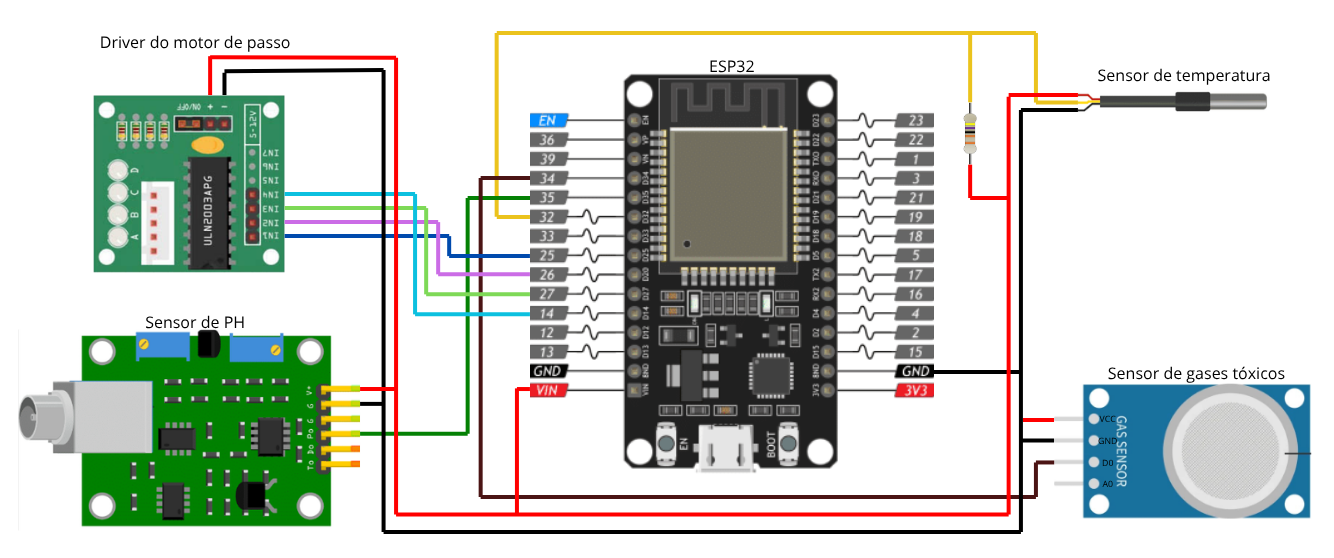
\includegraphics[width=1.0\linewidth]{imgs/diagrama-iot-camarize.png}
\caption{Diagrama referente a montagem do componente IoT}
\label{fig:iot_diagrama}
\end{figure}
 
O ciclo de leitura dos parâmetros e a transmissão dos pacotes via \textit{Wi-Fi} para a nuvem ocorrem em intervalos regulares de 1 minuto, visando manter um monitoramento contínuo adequado para a análise do cativeiro e evitar a sobrecarga no banco de dados. O ESP32 envia as leituras à API, que as registra no banco de dados. O firmware não armazena leituras localmente durante interrupções de conectividade \textit{Wi-Fi}; as leituras do período em que a conexão está indisponível não são registradas.
 
O sensor de pH foi ajustado utilizando uma solução-padrão de pH 7,00. Durante o procedimento, o potenciômetro da placa de condicionamento de sinal foi ajustado manualmente com uma chave de fenda, utilizando a solução como referência.
 
O controle da alimentação é realizado de forma integrada entre o ESP32 e a API. No horário programado, o ESP32 consulta a API para obter a configuração de dieta ativa do cativeiro, verificando o horário e a quantidade de ração definidos pelo usuário. Com base nessa resposta, o ESP32 aciona o motor do dispensador, libera a quantidade configurada e envia uma confirmação à API, que registra a alimentação realizada e notifica o usuário. Essa arquitetura garante que as configurações de alimentação sejam sempre gerenciadas de forma centralizada pela aplicação, permitindo que o usuário altere horários e quantidades remotamente sem necessidade de reconfiguração física do equipamento.
 
\subsection{Funcionalidades da Aplicação Web}
 
A interface da aplicação foi estruturada para oferecer ao produtor uma visão centralizada e intuitiva de seus cativeiros. A tela principal exibe todos os cativeiros cadastrados pelo usuário, permitindo a seleção individual de cada um para acesso às informações detalhadas. Ao acessar um cativeiro específico, o usuário visualiza os valores atuais de temperatura, pH e amônia coletados pelo ESP32 a cada minuto, acompanhados de gráficos históricos semanais que permitem identificar tendências e variações nas condições da água ao longo do tempo. Os limites ideais de cada parâmetro são definidos pelo próprio usuário no momento do cadastro do cativeiro, de acordo com as características da espécie cultivada e as condições locais de produção. Quando uma leitura ultrapassa os limites configurados, o sistema classifica automaticamente a severidade do desvio e aciona dois canais de alerta simultaneamente: uma notificação \textit{push} enviada diretamente ao dispositivo móvel do usuário e um e-mail com os detalhes do parâmetro fora do limite, garantindo que o produtor seja informado independentemente de estar com a aplicação aberta no momento do evento.
 
O controle da alimentação é realizado diretamente pela plataforma, onde o usuário define, para cada cativeiro, os horários das alimentações (o número de horários corresponde ao número de alimentações diárias) e a quantidade de ração por alimentação. Essas configurações são armazenadas no banco de dados em nuvem e utilizadas pelo ESP32 para acionar o dispensador, registrando cada alimentação realizada. O histórico de alimentações fica disponível na plataforma, permitindo ao produtor acompanhar se os ciclos de alimentação estão sendo executados corretamente ao longo do tempo.
 
O sistema contempla ainda diferentes níveis de acesso, com permissões distintas para cada perfil de usuário. O proprietário do cativeiro possui acesso completo às funcionalidades da plataforma, incluindo cadastro e gerenciamento de cativeiros, configuração de alertas e dietas, e visualização de relatórios. Funcionários cadastrados têm acesso restrito às informações operacionais, sem permissão para alterar configurações críticas do sistema. Essa estrutura de controle de acesso contribui para a segurança operacional e permite que múltiplos colaboradores utilizem a plataforma sem alterar as configurações definidas pelo proprietário.
 
\subsection{Validação dos Sensores}
\label{sec:validacao-sensores}
 
A validação foi realizada em um aquário dividido em duas seções independentes, uma com peixes e outra com camarões \textit{Macrobrachium rosenbergii}, sem compartilhamento de água entre elas, com um total de 8 camarões e 4 peixes adultos. Foram realizados seis testes, em diferentes condições de temperatura e pH. Os testes 1 e 6 foram realizados diretamente na água do cativeiro, em temperatura ambiente. Nos demais testes, para evitar risco aos animais, foram utilizadas amostras de água retiradas do cativeiro, mantidas em recipientes de plástico com tampa de 500 ml, para evitar a evaporação e a perda de gases dissolvidos, sendo um para a leitura do sensor de pH e outro para a do sensor de amônia. A temperatura das amostras foi reduzida por refrigeração em geladeira e elevada por exposição ao sol. O pH foi elevado com carbonato de sódio e reduzido com ácido clorídrico.
 
Em cada teste, os sensores permaneceram na amostra por 30 minutos, com leituras a cada 1 minuto, e o valor do sensor adotado foi a média das leituras do período; entre um teste e o seguinte houve um intervalo de 30 minutos. Os valores de referência foram obtidos simultaneamente, com instrumentos de uso aquarístico: o termômetro OceanTech ST-3, o kit colorimétrico de pH OceanTech High Precision (20 mL) e o kit colorimétrico de amônia Induspharma (30 mL). Por serem instrumentos de baixo custo, sua exatidão e resolução limitam a incerteza da comparação, o que é considerado na análise dos resultados. O MQ-135 foi posicionado no ar, acima da superfície da água, e mede a concentração do gás na fase gasosa; seus valores não são diretamente comparáveis aos do kit colorimétrico, que mede a amônia dissolvida na água.
 
\subsection{Análise dos Dados}
 
Para cada parâmetro, foram calculados, a partir do valor do sensor $s_i$ e do valor de referência $r_i$ no teste $i$ ($n = 6$), o erro $e_i = s_i - r_i$ e as métricas a seguir:
 
\begin{equation}
\bar{e} = \frac{1}{n}\sum_{i=1}^{n} e_i, \qquad
\mathrm{EAM} = \frac{1}{n}\sum_{i=1}^{n} |e_i|, \qquad
\mathrm{DP} = \sqrt{\frac{1}{n-1}\sum_{i=1}^{n}\left(e_i-\bar{e}\right)^2},
\end{equation}
 
\noindent em que $\bar{e}$ é o viés (erro sistemático), EAM é o erro absoluto médio e DP é o desvio-padrão do erro. Para comparação com a literatura, que reporta o desempenho em percentual, calculou-se também o erro percentual médio, $\mathrm{EPM} = \frac{100}{n}\sum_{i=1}^{n} |e_i|/r_i$, e a exatidão percentual, $100 - \mathrm{EPM}$. Como o erro percentual de temperatura e de pH depende da escala (graus Celsius, escala logarítmica de pH), as métricas em valores absolutos são as de referência neste trabalho.
 
A viabilidade técnica foi analisada pelos seguintes critérios: (i) para temperatura e pH, comparação das leituras do sensor com os valores dos instrumentos de referência; (ii) recebimento dos alertas pelo usuário nos dois canais e o tempo decorrido; (iii) operação contínua do ESP32 durante os testes; (iv) funcionamento das funcionalidades da aplicação web e do dispensador de ração.
 
\subsection{Processo de Avaliação do Sistema}
Além da validação dos sensores, o sistema foi avaliado em três frentes complementares: tempo de resposta do sistema de alertas, estabilidade operacional do componente IoT e funcionamento da aplicação web.
 
O tempo de resposta foi avaliado durante os seis testes de validação, observando o intervalo entre o recebimento da leitura pela API e a chegada da notificação \textit{push} e do correio eletrônico ao usuário.
 
A estabilidade operacional do ESP32 foi avaliada por observação ao longo dos testes (cerca de 5,5 horas), verificando o comportamento do dispositivo em operação contínua e sua resposta a uma interrupção de conectividade \textit{Wi-Fi} simulada por meio da troca do ponto de acesso à rede. Não houve registro sistemático de eventos nem da duração da interrupção.
 
O dispensador de ração foi acionado durante os testes, e sua avaliação considerou três critérios: execução do acionamento no horário programado, liberação da quantidade de ração configurada e registro do evento na plataforma.
 
A avaliação funcional da aplicação web foi conduzida em notebook e smartphones, abrangendo a visualização dos parâmetros, a exibição dos gráficos históricos, o recebimento de alertas automáticos e o controle remoto da alimentação. A avaliação de uso foi qualitativa e realizada pela equipe de desenvolvimento e pela proprietária do aquário, que auxiliou na condução dos testes coletando a água do aquário e disponibilizando o local para a realização dos testes.

% Resultados e Discussões
\section{Resultados e Discussões}

\subsection{Resultados da aplicação}

A aplicação web encontra-se em funcionamento em ambiente de produção. As funcionalidades de cadastro de usuários, gerenciamento de cativeiros, visualização de dados em painel de controle interativo, sistema de alertas automáticos e controle automatizado da alimentação foram implementadas e verificadas funcionalmente em notebook e smartphones. A avaliação de uso, realizada pela equipe de desenvolvimento e pela proprietária do aquário, indicou que a interface atende aos requisitos de navegabilidade e clareza; a avaliação com produtores é um trabalho futuro.

\subsection{Resultados dos testes com sensores}

Como referência para a interpretação dos resultados, foram consideradas as faixas aceitáveis de cultivo identificadas na pesquisa de campo: temperatura entre 25°C e 30°C e pH entre 6,5 e 8,5 e amônia abaixo de 0,1 ppm, parâmetro não medido pelo sistema. Os testes incluíram condições dentro e fora dessas faixas, a fim de avaliar o comportamento dos sensores em cenários distintos.

A Tabela \ref{tab:sensores} apresenta os resultados comparativos obtidos em cada um dos seis testes de validação, conforme a metodologia descrita na seção anterior.

\begin{table}[H]
\centering
\caption{Comparação entre valores de referência e leituras do sensor ESP32}
\begin{tabular}{ccccc}
\hline
\textbf{Teste} & \textbf{Temp. Real (°C)} & \textbf{Temp. Sensor (°C)} & \textbf{pH Real} & \textbf{pH Sensor} \\
\hline
1 & 21,0 & 20,50 & 7,0 & 6,79 \\
2 & 26,0 & 25,79 & 7,0 & 6,79 \\
3 & 17,0 & 16,80 & 7,0 & 6,79 \\
4 & 21,0 & 20,50 & 5,0 & 4,80 \\
5 & 22,0 & 21,60 & 8,6 & 7,90 \\
6 & 22,0 & 21,60 & 7,0 & 6,79 \\
\hline
\textbf{Erro percentual médio} & \multicolumn{2}{c}{\textbf{1,73\%}} & \multicolumn{2}{c}{\textbf{4,02\%}} \\
\textbf{Precisão média} & \multicolumn{2}{c}{\textbf{98,27\%}} & \multicolumn{2}{c}{\textbf{95,98\%}} \\
\hline
\end{tabular}

\vspace{2mm}
{\small Erro percentual = |sensor $-$ referência| / referência; precisão média = 100\% $-$ erro percentual médio. Testes 1 e 6 no cativeiro; demais em amostras (Seção~\ref{sec:validacao-sensores}).}
\label{tab:sensores}
\end{table}

O sensor de temperatura apresentou erro absoluto médio de 0,37°C (desvio-padrão de 0,13°C) ao longo dos seis testes, cobrindo uma faixa de 17,0°C a 26,0°C, o que corresponde a um erro percentual médio de 1,73\% e a uma precisão média de 98,27\%. Em todos os testes o sensor registrou valores abaixo da referência (viés de $-0{,}37$°C), com erros absolutos não superiores a 0,5°C. Por a referência ser um termômetro de uso aquarístico, o resultado indica compatibilidade entre as leituras, e não exatidão absoluta do sensor.

O sensor de pH apresentou erro absoluto médio de 0,29 (desvio-padrão de 0,20), correspondente a um erro percentual médio de 4,02\% e a uma precisão média de 95,98\%. Em todos os testes o sensor registrou valores abaixo da referência: nos testes 1, 2, 3 e 6 (referência 7,0) registrou 6,79 e, no teste 4 (referência 5,0), registrou 4,80, diferenças de 0,21 e 0,20, praticamente constantes, o que indica um desvio sistemático e não uma imprecisão aleatória. Como o sensor foi ajustado em solução-padrão de pH 7,00 antes dos testes, a origem desse desvio pode estar no sensor ou na resolução do kit colorimétrico de referência, e os dados disponíveis não permitem distingui-la.

A maior divergência ocorreu no teste 5, em que o pH foi elevado para 8,6 com carbonato de sódio em recipiente separado: o sensor registrou 7,90, diferença de 0,70 (8,14\%). Entre as possíveis causas estão a homogeneização incompleta da solução e o fato de o ajuste do sensor ter sido feito apenas em pH 7,00, o que pode comprometer a leitura em valores distantes dessa referência; essas hipóteses não foram testadas.

O sensor MQ-135 não registrou detecção de amônia em nenhum dos testes, e o kit colorimétrico também indicou ausência do composto, já que a água do aquário havia sido trocada no dia dos testes. Esse resultado não valida o sensor: o MQ-135 é um sensor de gases projetado para o ar, e não para a amônia dissolvida na água, e não foi exposto a amônia em concentração conhecida, de modo que não há evidência de que responderia a ela. A validação do monitoramento de amônia permanece como limitação, exigindo um sensor apropriado ao meio aquático.

O protótipo do dispensador de ração foi acionado nos seis testes de validação, com o acionamento ocorrendo nos horários programados e o registro do evento na plataforma realizado com êxito em todas as execuções.

\subsection{Tempo de Resposta do Sistema de Alertas}
Em todos os seis testes de validação, o ESP32 enviou as leituras à API no ciclo regular de 1 minuto. A API avalia cada leitura no momento em que a recebe e, quando um limite é ultrapassado, dispara o alerta de imediato, de modo que o usuário recebeu a notificação \textit{push} e o e-mail sem atraso perceptível após a chegada da leitura. O atraso máximo entre a ocorrência do evento e o alerta fica, portanto, limitado ao intervalo de leitura de 1 minuto, compatível com a rotina descrita pelos participantes da pesquisa de campo, que verificam a água de três a quatro vezes por dia.

\subsection{Estabilidade Operacional do ESP32}
O ESP32 operou de forma contínua ao longo dos testes, totalizando cerca de cinco horas e meia de funcionamento, sem reinicializações observadas. Durante esse período, foi simulada uma interrupção de conectividade \textit{Wi-Fi} por meio da troca do ponto de acesso à rede. Após o restabelecimento da conexão, o envio das leituras foi retomado. Como o firmware não armazena leituras localmente, as leituras do período de interrupção não foram registradas, o que constitui uma limitação do sistema atual.

% Conclusão
\section{Conclusão}

O presente trabalho apresentou o desenvolvimento e a validação de um sistema de monitoramento e automação voltado à carcinicultura, com o propósito de suprir a carência tecnológica observada no manejo dos cativeiros no Vale do Ribeira. O resultado é uma solução composta por uma aplicação web progressiva e um \textit{hardware} IoT baseado no microcontrolador ESP32, cuja viabilidade técnica foi indicada em testes de bancada, com limitações que fazem com que o objetivo geral tenha sido parcialmente alcançado.

Quanto aos objetivos específicos, o monitoramento remoto com emissão de alertas foi parcialmente alcançado: os alertas foram recebidos pelo usuário nos dois canais e os sensores de temperatura e pH apresentaram precisão média de 98,27\% e 95,98\%, respectivamente, com leituras sistematicamente abaixo da referência; o monitoramento de amônia, porém, não foi validado, pois o sensor MQ-135, projetado para gases no ar, não registrou detecção e não foi exposto a amônia em concentração conhecida. O registro de dados históricos, com gráficos e relatórios, foi implementado e funcionou na plataforma, cumprindo o segundo objetivo. A automação do fornecimento de ração foi alcançada: o acionamento nos horários programados e o registro na plataforma ocorreram. Por fim, a aplicação web responsiva foi desenvolvida e oferece ao produtor acesso remoto aos parâmetros monitorados e à configuração da alimentação, sem necessidade de instalação nativa.

A respeito das limitações de \textit{hardware} e da inerente dependência de conectividade \textit{Wi-Fi}, o projeto estabelece uma base tecnológica escalável. Como trabalhos futuros, planejam-se intervenções focadas na robustez física: a substituição do módulo de amônia por um sensor íon-seletivo submersível e a validação integral do protótipo em ambiente comercial de cativeiro. Com essas evoluções, o sistema continuará sua trajetória para se consolidar como uma ferramenta acessível e viável para a modernização do mercado produtor de camarões.

O sistema apresenta como limitações a dependência de conectividade \textit{Wi-Fi}, a ausência de armazenamento local das leituras durante interrupções, a validação restrita a um aquário, a uma espécie e a cerca de cinco horas e meia de operação, e o uso de instrumentos de referência de baixo custo. Como trabalhos futuros, planejam-se a substituição do módulo de amônia por um sensor íon-seletivo submersível, o armazenamento local das leituras e a validação integral do protótipo em ambiente comercial de cativeiro.

% Referências
\bibliographystyle{IEEEtran}
\bibliography{referencias}

\end{document}
